\chapter{El problema inverso}%
\lhead{\thepage}
\rhead{\textit{El problema inverso}} \\
\vspace{0.01\textheight}
\label{sec:inverso}
%\pagebreak

En las secciones previas abordamos el problema directo de transporte 
de radiación en la materia mediante la ETR. En síntesis, el problema 
directo consta de, dados los parámetros ópticos $a(\x)$, $b(\x)$, la función  
de fase $\eta(\hth\cdot \hth')$, la velocidad de la luz en el medio participante 
$c$, las fuentes internas $s$ y las condiciones iniciales y de contorno, 
encontrar la solución $\ut$ a la ecuación~\eqref{eq:RTE}.

Para el problema inverso en tomografía óptica, alguno de los parámetros 
ópticos es desconocido, 
o conocido sólo parcialmente, y se dispone de mediciones experimentales 
de detectores colocados en el contorno del dominio que se quiere analizar. 
A partir de las mediciones experimentales de estos detectores, 
el objetivo es la reconstrucción de uno o más de los parámetros ópticos. 
En el caso de tomografía por fluorescencia y tomografía de bioluminiscencia, lo que se intenta reconstruir 
son las fuentes $s$ en la ec.~\eqref{eq:RTE}~\cite{Klose2005,Klose2009,Ren2010}, 
que vienen relacionadas a los coeficientes de absorción de los 
cromoforos y fluoroforos. 

En el contexto de esta tesis, nos limitaremos a la reconstrucción del 
coeficiente de absorción, $a(\x)$. La reconstrucción de dicho coeficiente 
encuentra aplicaciones en tomografía de fluorescencia, y en tomografía óptica. 
La reconstrucción de las propiedades de absorción en tomografía óptica 
 permite la identificación de tumores~\cite{Zhu2005,Zhu2010,Fujii2016b}, 
la obtención de imagenes funcionales del cerebro humano~\cite{Boas2001,bluestone2001,Arridge1999}, 
y la caracterización de diferentes constituyentes del tejido 
humano para la obtención de imágenes en medicina. En 
este trabajo nos enfocamos en la reconstrucción del coeficiente 
de absorción, pero los algorítmos y las estrategias propuestas 
pueden ser fácilmente generalizadas para la reconstrución 
de otros parámetros. 

Generalmente, para aplicaciones 
en diágnostico y monitoreo en el tratamiento de tumores, 
se asume cierta información previa 
para el coeficiente de dispersión, 
$b(\x)$, obtenida por técnicas de obtención 
de imagenes de alta resolución~\cite{Althobaiti2017,Guven2003} \eg Resonancia Magnética. 
Este conocimiento previo obtenido por otras técnicas, también brinda 
información límitada en el parámetro óptico de absorción $a(\x)$, 
como pueden ser los coeficientes de absorción para ciertos tejidos óseos, 
o el aire en regiones como la traquea del cuello humano, como también 
se conocen cotas superiores e inferiores para dicho parámetro, 
lo que permite restringir el espacio de funciones donde se busca minimizar 
la función objetivo. El uso de técnicas de alta resolución, como la Resonancia 
Magnética, posee ciertas límitaciones, como el alto costo, la baja disponibilidad 
de este tipo de aparatos 
(lo que impone una dificultad a la hora de seguir la evolución de un tratamiento 
asistido por diagnóstico de imágenes), y adicionalmente los dispositivos 
utilizados en tomografía óptica son portables, lo que permite tenerlos disponibles 
para su uso en diversas situaciones. En la figura~\ref{fig:esquemainv} esquematizamos los problemas directos e inverso, tal como son 
tratados en esta tésis. 


\begin{figure}[h!]
\centering
  \includegraphics[width=\linewidth]{figuras/inv.pdf}\\
  \caption{
Grafico esquematico de los problemas directo e inverso, tal como son considerados 
en esta tésis.}
 \label{fig:esquemainv}
\end{figure}
Para la resolución del problema inverso, utilizamos el esquema \textit{MOBIR}, 
presentado en la sección siguiente. 

\section{El esquma \textit{MOBIR}}

\begin{wrapfigure}{l}{0.48\textwidth}
  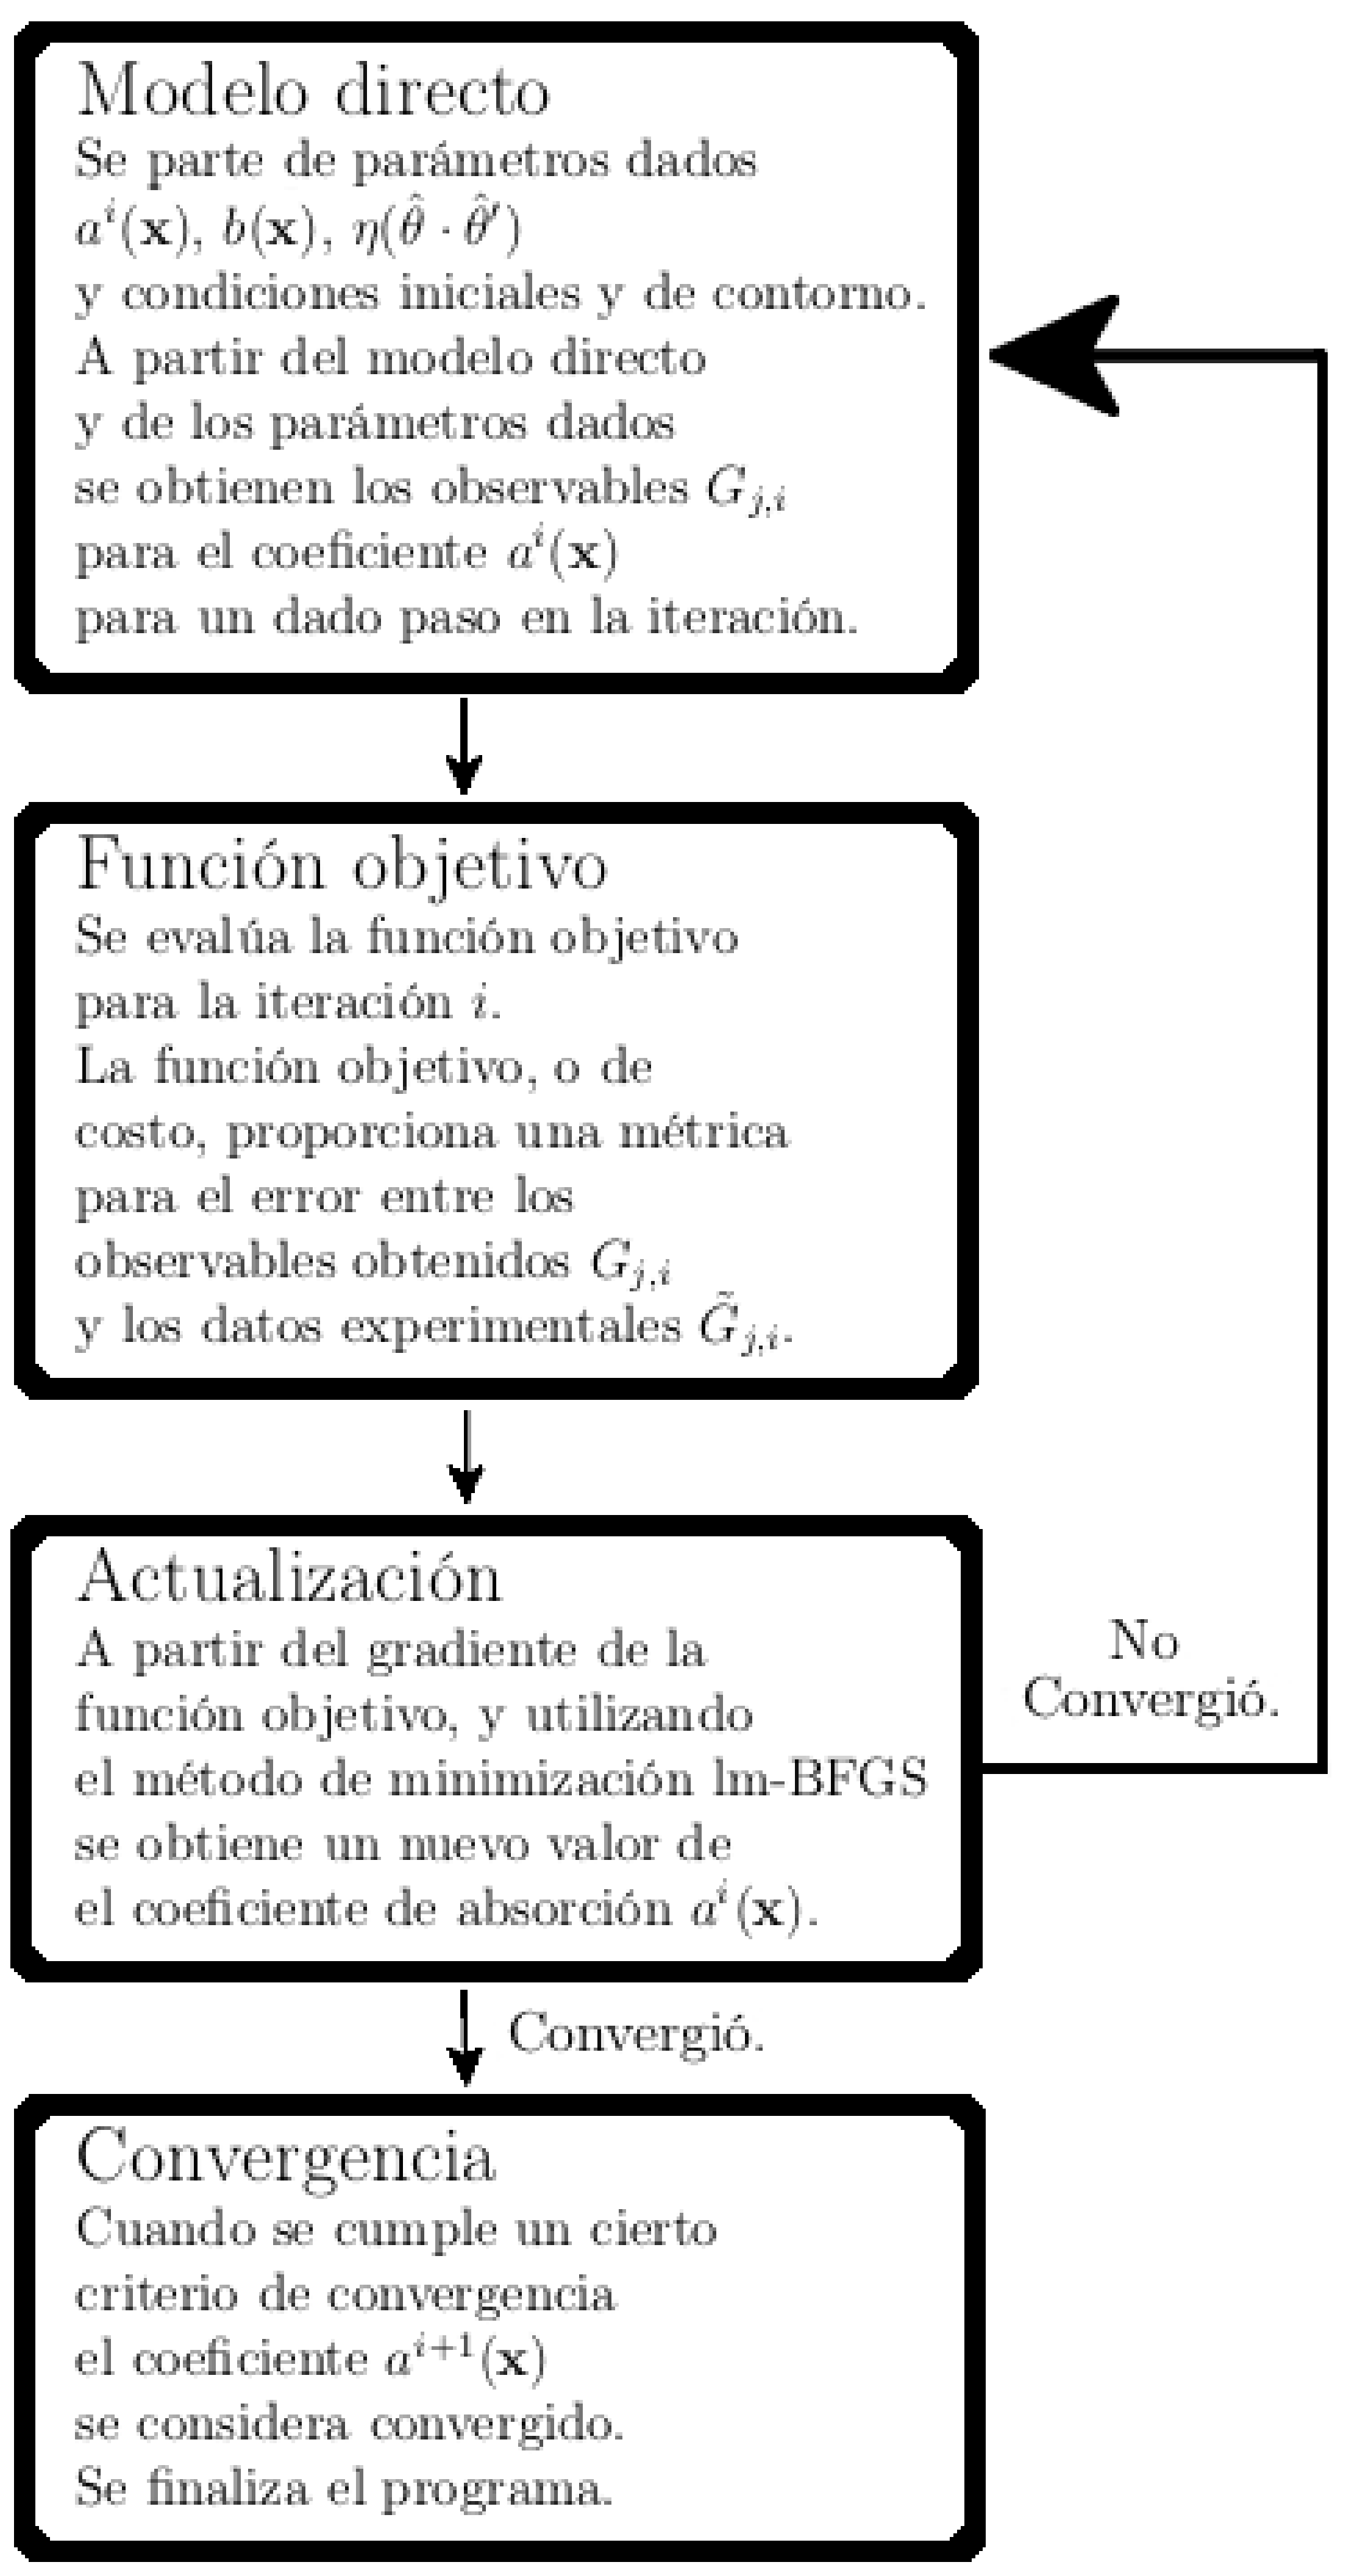
\includegraphics[width=0.48\textwidth]{figuras/mobir.eps}\\
  \caption{Esquema  MOBIR. El modelo directo es utilizado para obtener los observables simulados. Se evalúa el error entre los datos experimentales y los simulados por medio de la función objetivo. 
  Luego, utilizando un método de minimización, se actualiza el coeficiente $a(\x)^{i+1}$ a 
  ser utilizado en la iteración subsiguiente, hasta cumplir 
  un cierto criterio de convergencia. }
 \label{fig:mobir}
\end{wrapfigure}

En este tesis desarrollamos un algoritmo tipo MOBIR~\cite{Hielscher1999,Kim2010} (del inglés, {\em Model Based Iterative Image  
Reconstruction}). Este tipo de esquemas se basan en un modelo físico, y un método de minimización 
iterativo para la reconstrucción del parámetro deseado en el problema inverso.

El modelo físico utilizado es la Ecuación de Transporte Radiativo~\eqref{eq:RTE}. 
Para la minimización del funcional objetivo (que será introducido en una sección posterior) emplearemos el método de minimización 
de Broyden–Fletcher–Goldfarb–Shanno (BFGS) con uso de memoria reducido 
(lm-BFGS, de su sigla en inglés)~\cite{Byrd1995}. 

El problema inverso en tomografía óptica es resuelto como un problema de optimización 
no lineal. A partir de un valor inicial para el coeficiente de absorción $a(\x)^0$, 
el coeficiente de absorción es buscado de forma iterativa, actualizando su valor 
en cada iteración mediante el método lm-BFGS, el cual es un caso particular 
de los métodos de cuasi-Newton~\cite{Nocedal2006,Klose2003QN,Ren2006}. 
Partiendo del valor inicial $a^0(\x)$, el cual en general es estimado 
a partir de información obtenida de manera previa por otros métodos de imagenes, 
el coeficiente de absorción es 
\clearpage
\noindent actualizado en cada paso de la iteración $i+1$, según~\cite{Klose2003QN}
\begin{equation}
\mathbf{a}^{i+1}(\x)=\mathbf{a}^{i}(\x)+\alpha^i  \mathbf{d}^i(\x)
\label{eq:update}
\end{equation}
donde $\mathbf{a}^{i}(\x)$ debe ser interpretado como el 
vector obtenido a partir de el coeficiente de absorción en el 
dominio espacial $\Omega$  
discretizado, con $\alpha^i$ el largo del paso de Newton (que lo consideraremos 
en general $\alpha^i=1$), y $\mathbf{d}^i(\x)$ 
la dirección de descenso. En el caso del método de Newton (o {\em steepest descent}), la dirección de 
descenso vendrá dada por el gradiente $\mathbf{d}^i=-\nabla_a $ de la función objetivo $g$ (que será definida posteriormente). 
En el contexto de esta tesis emplearemos el método lm-BFGS, ya que este método a 
mostrado ser eficiente en el contexto de tomografía óptica~\cite{Klose2003QN,Ren2006,
Prieto2017}. 

\section{El método de minimización BFGS}
\label{sec:BFGS}
Siguiendo a Nocedal~\cite{Nocedal2006}, el método BFGS parte de considerar la expansión de Taylor a segundo orden de la función objetivo 
que buscamos minimizar, la cual estará evaluada para el coeficiente $\mathbf{a}(\x)$,  
lo notaremos, por simplicidad  $g[\mathbf{a}]$

\begin{equation}
g[\mathbf{a}^i+ \mathbf{d}^i]\approx g[\mathbf{a}^i]+ (\mathbf{d}^i)^T \nabla_a g[\mathbf{a}^i]+\frac{1}{2}(\mathbf{d}^i)^T \nabla_a^2 g[\mathbf{a}^i+t\mathbf{d}^i] \mathbf{d}^i=m(\mathbf{d}^i).
\label{eq:Taylor}
\end{equation}
donde $t \in (0,1)$, y $(\mathbf{d}^i)^T$ indica el vector traspuesto a $\mathbf{d}^i$.
Además, si $g$ es al menos dos veces diferenciable se cumple qué 
\begin{equation}
\nabla_a g[\mathbf{a}^i+ \mathbf{d}^i]\approx \nabla_a g[\mathbf{a}^i]+\int_0^1\nabla_a^2 g[\mathbf{a}^i+t\mathbf{d}^i] \mathbf{d}^idt 
\label{eq:Taylor2}
\end{equation}
para algún $t \in (0,1)$.
Exigiendo que se anule la derivada de $m(\mathbf{d^i})$, se llega la dirección de Newton, dada por
\begin{equation}
\mathbf{d}^i=-(\nabla_a^2 g^i )^{-1} \nabla_a g^i.
\label{eq:direccion}
\end{equation}
El principal obstaculo para la aplicación de la dirección de Newton es la 
necesidad de calcular la inversa del Hessiano de la función objetivo, $\nabla_a^2 g^i$, 
lo cual en tomografía óptica, debido a la alta dimensionalidad de la ETR, puede 
resultar extremadamente costoso. 

Por este motivo, el método BFGS implementa una aproximación del Hessiano de la función objetivo (mas concretamente, 
a la inversa del Hessiano) que 
es actualizada a cada paso de la iteración. Sumando y restando el término $ \nabla_a^2 g \mathbf{d}^i$ en la ecuación~\eqref{eq:Taylor2} se llega a
\begin{equation}
\nabla_a g[\mathbf{a}^i+ \mathbf{d}^i]\approx \nabla_a g[\mathbf{a}^i]+ \nabla_a^2 g[\mathbf{a}^i]\mathbf{d}^i + \int_0^1   \left( \nabla_a^2 g[\mathbf{a}^i+t\mathbf{d}^i]-\nabla_a^2 g[\mathbf{a}^i] \right)\mathbf{d}^idt
\label{eq:Taylor3}
\end{equation}
Dado que se asume la continuidad de $\nabla_a g$, el término de la integral 
es $o(||\mathbf{a}^{i+1}-\mathbf{a}^{i}||)$. Tomando $\mathbf{d}^i=\mathbf{a}^{i+1}-\mathbf{a}^{i}$ se llega a la relación
\begin{equation}
\begin{split}
\begin{aligned}
\nabla_a g[\mathbf{a}^{i+1}] &\approx \nabla_a g[\mathbf{a}^i]+ \nabla_a^2 g[\mathbf{a}^{i+1}-\mathbf{a}^i]  + o(||\mathbf{a}^{i+1}-\mathbf{a}^{i}||).\\
\therefore \nabla_a^2 g[\mathbf{a}^{i+1}-\mathbf{a}^i]& \approx \nabla_a g[\mathbf{a}^{i+1}]  - \nabla_a g[\mathbf{a}^{i}].
\end{aligned}
\end{split}
\label{eq:Taylor4}
\end{equation}
Esta última relación nos permite aproximar el Hessiano utilizando las derivadas de 
la función objetivo obtenidos para dos iteraciones sucevias. 
La inversa del Hessiano de la función objetivo es aproximada exigiendo que se cumpla la última relación en~\eqref{eq:Taylor4}, que puede escribirse 
\begin{equation}
(B^{i+1})^{-1}y^i=s^i,
\label{eq:Taylor5}
\end{equation}
con $s_i=  \mathbf{a}^{i+1}-\mathbf{a}^{i}$ y $y^i=\nabla_a g[\mathbf{a}^{i+1}]  - \nabla_a g[\mathbf{a}^{i}]$. La fórmula BFGS para actualizar el Hessiano en cada iteración viene dada por~\cite{Nocedal2006}
\begin{equation}
(B^{i+1})^{-1}=(V^i)^T (B^{i})^{-1}V^i + \rho^i s^i (s^i)^T  ,
%B^{i}-\frac{B^{i}s^i (s^i)^T B^i }{(s^i)^TB^i s^i}+ \frac{y^i (y^i)^T}{(y^i)^T s^i}
\label{eq:HBFGS}
\end{equation}
la cual cumple la relación~\eqref{eq:Taylor5}, donde $\rho^i=\frac{1}{(y^i)^T s^i}$ 
y $V^i=\id - \rho^i y^i (s^i)^T$. 
La dirección de descenso, finalmente, se obtiene de la ecuación~\eqref{eq:direccion} reemplazando 
el Hessiano por su aproximación $B^i$
\begin{equation}
\mathbf{d}^{i}=-(B^{i})^{-1} \nabla_a g[\mathbf{a}^i]. 
\label{eq:HBFGS}
\end{equation}

\subsection{El método de uso de memoria limitada lm-BFGS}
\label{sec:lmBFGS}
En nuestro algoritmo para la resolución del problema inverso, el coeficiente 
de absorción es actualizado en cada iteración utilizando la relación 

\begin{equation}
\mathbf{a}^{i+1}(\x)=\mathbf{a}^{i}(\x)-(B^{i})^{-1} \nabla_a g[\mathbf{a}^i]
\label{eq:update2}
\end{equation}
Debido a que la aproximación a la inversa del Hessiano, $(B^i)^{-1}$, en tomografía óptica es una matriz 
que para el problema 2D discretizado, con $N_x \times N_y$ puntos 
por cada coordenada espacial tendrá dimensiones  $B^i\in \mathbb{R}^{N_x \times N_y}$, 
la manipulación y almacenamiento de esta matriz puede ser sumamente costosa. Por ello, 
para evitar la manipulación y el almacenamiento de esta matriz, se utiliza 
una versión aproximada de $(B^i)^{-1}$, para la cual se almacenan los vectores $\{s^k, y^k\}$, 
$k=i-m,...,i-1$ para un dado número de puntos $m$ previos a la iteración $i$-esima. 
Para esto se utiliza una aproximación inicial al Hessiano $(B^i)^{-1}_0$
\begin{equation}
(B^i)^{-1}_0=\gamma^i \id,\quad \quad \gamma^i=\frac{(s^{i-1})^T y^{i-1}}{(y^{i-1})^Ty^{i-1}},
\label{eq:initHess}
\end{equation}
y utilizando la ecuación~\eqref{eq:HBFGS} se tiene la relación de recurrencia
\begin{equation}
\begin{split}
\begin{aligned}
(B^{i+1})^{-1}=&(V^{i-1})^T...V^{i-m})^T) (B^i)^{-1}_0 (V^{i-m}...V^{i-1})  \\
&+\rho^{i-m} (V^{i-1})^T...V^{i-m+1})^T)s^{i-m} (s^{i-m})^T(V^{i-m+1}...V^{i-1+1}) \\
&+\rho^{i-m+1} (V^{i-1})^T...V^{i-m+2})^T)s^{i-m+1} (s^{i-m+1})^T(V^{i-m+2}...V^{i-1}) \\
&+...\\
&+\rho^{i-1} s^{i-1} (s^{i-1})^T. 
\end{aligned}
\end{split}
\label{eq:HBFGSrec}
\end{equation}
de donde se tiene el algoritmo~\eqref{algbfgs}~\cite{Byrd1995,Nocedal2006}

\begin{algorithm}
\caption{lm-BFGS}\label{algbfgs}
\begin{algorithmic}[1]
\State dados $m$, $\mathbf{a}^i$, y $\nabla_a g[\mathbf{a}^i]$
\State  $q = \nabla_a g[\mathbf{a}^i]$
\State \textbf{para} $k=i-1,i-2,\ldots,i-m$ hacer 
\State \hskip 0.75em $\alpha^k  = \rho^k (s^k)^T q$,
\State \hskip 0.75em $q  = q- \alpha^k y^k$,
\State \textbf{terminar}
\State $r = (B_0^k)^{-1} q$,
\State \textbf{para} $k=i-m,i-m+1,\ldots,i-1$ hacer 
\State \hskip 0.75em $\beta  = \rho^k (y^k)^T r$,
\State \hskip 0.75em $r  = r+s^k(\alpha^k-\beta)$,
\State \textbf{terminar}
\State Finalizar programa, con $(B^k)^{-1}\nabla_a g[\mathbf{a}^k]=r$.
\end{algorithmic}
\end{algorithm}  
  
En esta tesis utilizaremos el algoritmo lm-BFGS para encontrar 
el mínimo de la función objetivo. En todos los casos, usaremos el valor 
de $m=5$, y se parte de un coeficiente inicial $a^0(\x)$ dado 
por cierto conocimiento obtenido previamente, como puede ser la imagen 
de resonancia magnética de un cuello humano utilizada en la sec.~\ref{sec:inverseres}.
Adicionalmente, es posible incluir cotas para el coeficiente 
de absorción que deseamos reconstruir, de forma tal que 
el proceso de minimización sea realizado 
en un subespacio tal que $a^l(\x)\leq a^i(\x) \leq a^u(\x)$, de forma 
tal que el coeficiente de absorción, para cada punto espacial $\x$ se encuentre 
restringido por las cotas inferior $a^l(\x)$ y superior $a^u(\x)$. Esto restringe el espacio de soluciones posibles, permitiendo explotar información a priori obtenida por otros métodos de imágenes. 
Una condición física que debe cumplirse siempre es que la cota inferior 
para el coeficiente de absorción cumpla $a^l(\x)\geq 0$. Similarmente, 
se conocen cotas superiores para el coeficiente de absorción, y además, 
puede utilizarse los valores conocidos de $a(\x)$ como cotas sobre 
aquellos tejidos donde se sabe que la inclusión no puede ocurrir, 
o si, por la naturaleza del diagnóstico que se está realizando, 
se espera que una dada inclusión 
se encuentre dentro de cierto tipo de tejido, restringiendo mediante cotas 
la reconstrucción para que ocurra dentro del tejido esperado, fijando los 
valores para el resto de los tejidos, como puede ser, la existencia de 
una región de absorción y dispersión nula en la traquea para el cuello 
humano, o las regiones óseas para el caso en el que se intenta dar un diagnóstico 
para un tipo de tumor específico, como lo puede ser para el cáncer de tiroides, 
donde se sabe que el tumor se encontrará localizado en el tejido blando. 
El procedimiento por el cual se imponen dichas cotas en los coeficientes 
puede encontrarse en la ref.~\cite{Byrd1995}. 

\section{El operador de transporte y otras definiciones preliminares}
En esta sección, haremos uso del operador de transporte, el cual definimos
según
\begin{equation}
\begin{split}
\mathcal{T}[u]=\frac{1}
{c}\frac{\partial \ut}{\partial t} + \hth \cdot \nabla \ut&+a(\x)\ut\\
&+b(\x)\left[\ut - \int_{S^1}\eta(\hth\cdot\hth ') u(\x,\hth',t) d\theta'\right],
\end{split}
\label{eq:Toper}
\end{equation}
donde se hizo explícita la dependencia del operador de transporte \mathcal{T} 
con respecto a $\ut$. 

Consideramos el problema ETR de valores iniciales y condiciones 
de contorno
\begin{equation}
\begin{split}
\begin{aligned}
&\mathcal{T}\big[u\big]=0, \;  (\x,\theta)  \in \Omega\times S^1\\
&u(\x,\hth,t=0)=0, \;  (\x,\theta)  \in \Omega\times S^1 \\
&u(\x,\hth,t)=f(\hth \cdot \hnu) u(\x,\hth_r,t) + q(\x,\hth,t) , \; (\x,\hth) \in \Gamma_-
\end{aligned}
\end{split}
\label{eq:RTEt}
\end{equation}
donde todas las cantidades fueron definidas en la sección~\ref{sec:ETR}.


Para concluir esta sección, mencionamos la ``función ventana''~\cite{Bruno2014}
\begin{equation}
\begin{aligned}
\begin{split}
w(v)=
\begin{cases}
  1 &\text{for} \, \, v = 0, \\
       \exp{\left(\frac{2e^{-1/|v|}}{|v|-1}\right)} & \text{for} \, \, 0 < |v| < 1, \\
       0 &\text{for} \, \, |v| \geq 1.
     \end{cases}
\end{split}
\end{aligned}
\label{eq:sourcelabwind}
\end{equation}
de la variable real $v$, la cual se anula para $|v|\geq 1$ y realiza 
una transición suave a uno en el intervalo $-1 < v < 1$. Esta función 
será utilizada de diferentes formas en las secciones subsiguientes---
incluyendo el modelado del perfil temporal y ángular de los pulsos láser, 
así como el modelado de la sensibilidad espacial de los fotodetectores.
\begin{figure}[h!]
\centering
  \includegraphics[width=0.5\linewidth]{figuras/windowed.eps}
  \caption{Grafico de la función ventana $w(v)$~\eqref{eq:sourcelabwind} utilizada 
  para modelar los perfiles temporales y ángular de las fuentes láser, 
  así como la sensibilidad espacial de los fotodetectores.}
 \label{fig:parallelgeom}
\end{figure}


\section{El método de Fuentes Múltiples Superpuestas}
\label{sec:FMS}
El problema inverso en tomografía óptica en el dominio temporal, es ubicuamente resuelto utilizando el denóminado ``método de barrido'' (MB), del inglés, ``Transport Sweep''. En éste método, se requiere la resolución de un problema directo y un problema adjunto 
para cada fuente $q_i(\x,\hth,t)$, $i=1,\ldots,N_q$ en la ecuación~\eqref{eq:RTEt}, 
con $N_q$ el número total de fuentes empleadas. 
El mayor inconveniente que encuetra este método es que el costo computacional 
incrementa linealmente con el número de fuentes utilizadas. En general, 
cada fuente permite sensar diferentes partes del dominio espacial en consideración. 
Dado que la intensidad lumínica de las fuentes laser empleadas sufre una 
atenuación de tipo exponencial, debido a la absorción y a la dispersión 
en el interior del medio participante, en general se requiere la utilización de 
fuentes múltiples. Debido a la atenuación exponencial de la intensidad lumínica, 
en general, la iluminación entre fuentes lejanas no suele afectarse entre sí. 
Motivados por este hecho en esta tesis introducimos un método de Fuentes Múltiples 
Simultáneas (FMS). Este método se vale del uso de ``fuentes generalizadas'', 
las cuales pueden representar una o múltiples fuentes láser, las cuales 
pueden ser activadas, con ciertos retrasos temporales, de forma superpuesta 
en un único problema directo, lo que brinda ventajas en el costo computacional 
que serán demostradas mas adelante.  

Los métodos MB y FMS se basan en el uso de dos tipos diferentes de fuentes, 
donde ambas pueden expresarse como
\begin{equation}
  q = q_i(\x,\hth,t) =\sum_{k=1}^{N_s} s_{k,i}(\x,\hth,t) ,\quad i=1,2,\ldots,N_q
\label{eq:RTEsources}
\end{equation}
para ciertos valores enteros de $N_q$ y $N_s$. Utilizando la 
función ventana~\eqref{eq:sourcelabwind}, definimos
\begin{equation}
  s_{k,i}(\x,\hth,t) = \exp(-|\x-\x_{k,i}|^2/
  2\sigma_\x^2)w(\beta_{k,i})w(\gamma_{k,i}),
\label{eq:RTEsources2}
\end{equation}
para las posiciones de las fuentes láser $\x_{k,i}\in\partial\Omega$, 
con el diámetro de la iluminación láser sobre la superficie del dominio $\partial \Omega$ 
siendo $\sigma_\x$, y la distribución 
ángular $\beta_{k,i}=|\theta-\theta_{k,i}|/\sigma_{\theta}$, 
donde $\theta_{k,i}$ ($0\leq \theta_{k,i} < 2\pi$) y $\sigma_{\theta}$
modelan el ángulo para la dirección $\hth_{k,i}$ en la que apunta el láser 
y la distribución ángular de la radiación para el láser $(k,i)$-ésimo, respectivamente. 
Similarmente, $\gamma_{k,i}=|t-\tau_{k,i}|/\sigma_t$, modela el pulso 
láser, con retardos temporales $\tau_{k,i}\geq 0$ para diferentes fuentes láser, 
y donde $\sigma_t$ denota la mitad de la duración total del pulso láser. 

Para las fuentes en el método MB fijamos $N_s=1$ y, en general, $N_q>1$ 
(se utiliza una secuencia de $N_q>1$ fuentes láser, requiriendo la resolución de 
$N_q$ pares de problemas directos y adjuntos por cada iteración en el problema inverso), 
mientras que en el método FMS propuesto, utilizamos $N_s>1$ y $N_q=1$ (de forma 
que $N_s>1$ fuentes laser son superpuestas en una única ``fuente generalizada'', 
requiriendo por lo tanto la resolución de un único par de problemas directo y 
adjunto por iteración para la resolución del problema inverso). En cada ``barido''
del método MB cada una de las $N_q>1$ fuentes laser es aplicada de forma 
independiente de las otras, con todos los retardos temporales $\tau_{i,1}=0$ ($1\leq i\leq N_q$), y se guardan los valores registrados por todos los fotodetectores utilizados~\cite{Prieto2017,Dorn}. En el método FMS propuesto, en cambio, 
se utiliza una única fuente generalizada ($N_q=1$), la cual incorpora 
las contribuciones de las $N_s>1$ fuentes laser alrededor de $\partial \Omega$, 
con retardos temporales $\tau_{1,k}\geq 0$. Debido a los retardos temporales 
utilizados, en el método FMS se requieren simulaciones mas largas para la resolución de los problemas directo y adjunto, en comparación con las simulaciones requeridas 
para cada una de las $N_q>1$ fuentes en el método MB. Sin embargo, como se 
demuestra en la sección~\ref{sec:inverseres}, la estrategia de fuentes simultaneas 
permite obtener ganancias significativas en términos del costo computacional 
total para todo el proceso de inversión, sin detrmiento en la precisión de la 
reconstrucción obtenida. 

\section{La función objetivo y el formalismo del método adjunto para el cálculo de su gradiente}

Tanto el método MB como el método FMS se basan en el uso de  $N_d\geq 1$ detectores, 
donde el detector $j$-ésimo ($1\leq j\leq N_d$) ubicado en el punto 
$\x_j \in \partial \Omega$, queda caracterizado por el operador 
de medición $G_j=G_j[u](t)$ definido como 
\begin{equation}
  G_j[u]=\oint_{\partial \Omega}\int_{\hth \cdot \hnu>0}[1-f(\hth
  \cdot \hnu)]
  \hth \cdot \hnu 
  \times w\left( \frac{ |\x-\x_j |}{\sigma_d} \right) \ut
  d\theta dS
\label{eq:OpMed}
\end{equation}
para cualquier función $\ut$ definida en $(\x,\hth,t)\in\Omega\times S^1 \times [0,T] $. 
Utilizando la función~\eqref{eq:sourcelabwind}, y llamando $\sigma_d>0$ 
al área efectiva de los detectores, el factor $w( |\x-\x_j |/\sigma_d) $ 
caracteriza la sensibilidad espacial del detector $j$-ésimo, 
y $dS$ denota el elemento de área en $\partial \Omega$. 
Claramente, el operador de medición $G_j[u]$ cuantifica el flujo de fotones 
transmitidos a través de la superficie del detector. Para cada 
fuente generalizada $q_i$ tenemos un número $N_d$ de detecciones 
resueltas en el tiempo. El número y la ubicación de los detectores 
permanecen fijos durante el proceso de inversión. 

En vista de las consideraciones hechas previamente en la sección~\ref{sec:inverso}, 
en lo que sigue haremos explícita la dependencia del operador de transporte 
$\mathcal{T}$ y de la solución $u$ en la ecuación~\eqref{eq:Toper} 
con respecto al coeficiente de absorción $a=a(\x)$ , llamando 
\begin{equation}\label{eq:Toper_a}
  \mathcal{T}[u] = \mathcal{T}[u,a]= \mathcal{T}[u,a](\x,\hth,t)
\end{equation}
y
\begin{equation}\label{u_of_a}
  u=u[a]=u[a](\x,\hth,t),
\end{equation}
respectivamente.

Expresamos el problema inverso para el parámetro óptico  $a(\x)$ 
en términos del problema de minimización de la función objetivo
\begin{equation}
  \Lambda[a]=\sum_{i=1}^{N_q} g_i[u_i],
\label{eq:FObjpr}
\end{equation}
donde, para un dado coeficiente de absorción $a$,
\begin{equation}\label{ui_of_a}
  u_i = u_i[a] = u_i[a](\x,\theta,t)
\end{equation}
denota la solución $u=u_i$ de la ecuación~\eqref{eq:RTEt} con $q=q_i$ 
(donde se incluyó un detalle creciente de derecha a izquierda en la ecuación~\eqref{eq:FObjpr}
concerniente a la dependencie de $u_i$ en $a$, y las variables espaciales, angular y temporal), 
y donde, para un dado número de mediciones $N_q \times N_d$ en los detectores $\tilde{G}_{j,i}$ 
($N_d$ detecciones $\tilde{G}_{j,i}$ para cada una de las $N_q$ fuentes generalizadas $q_i$) 
y utlizando la ecuación~\eqref{eq:OpMed}, $g_i$ denota la funcional 
\begin{equation}
  g_i[u] = \frac{1}{2} \sum_{j=1}^{N_d} \int_0^T (G_j[u]-\tilde
  {G}_{j,i})^2 dt.
\label{eq:FObj}
\end{equation}
Para minimizar la función objetivo~\eqref{eq:FObjpr} utilizamos el algorítmo 
de descenso por gradiente 
lm-BFGS-b (ver ref.~\cite{Byrd1995} y secciones~\ref{sec:BFGS} y~\label{sec:lmBFGS}), 
el cual se basa en el uso de la derivada funcional $\frac{d\Lambda}{da} [a;\delta a]$ 
con respecto al coeficiente de absorción $a = a(\x)$ en la dirección $\delta a$. 
Aquí notamos $\frac{d}{da}$ a la diferenciación de Gateaux~\cite{Hille1974}: 
para una dada función $a= a(\x)$ y una dada poerturbación $\delta a= \delta a(\x)$, 
la derivada de Gateaux de una dada funcional $h = h[a]$ en la dirección $\delta a$ 
se define según
\begin{equation}\label{gateaux}
  \frac{dh}{da}[a; \delta a ] = \lim_{\varepsilon \to 0} \frac{h[a +\varepsilon \delta a]
    - h[a]}{\varepsilon}.
\end{equation}
Puede darse una definición similar para las derivadas parciales de Gateaux 
de un operador $w = w[a](\x,\theta,t)$ (como, \eg, el operador~\eqref{eq:Toper}, 
la solución $u = u[a]=u[a](\x,\theta,t)$ a la ecuación~\eqref{eq:RTE},etc.):
\begin{equation}\label{gateaux_part}
  \frac{\partial w}{\partial a}[a; \delta a ](\x,\theta,t) = \lim_{\varepsilon \to 0} \frac{w[a +\varepsilon \delta a](\x,\theta,t)
    - w[a](\x,\theta,t)}{\varepsilon}.
\end{equation}
En lo que sigue, utilizamos las derivadas de Gateaux para la composición 
de funcionales y operadores, para los cuales se satisface la regla de la cadena. 
Por ejemplo, para la composición  $h\circ w [a] = h\big[w[a]\big]$ 
se tiene la deintidad de la regla de la cadena
\begin{equation}\label{eq:chain}
  \frac{d (h\circ w)}{da} \big[a;\delta a\big]= \frac{d h}{
    d w}\left[w[a];\frac{\partial w}{\partial a} \big[a;\delta
    a\big]\right].
\end{equation}
En nuestro contexto, podemos ilustrar esta relación como sigue. 
Al considerar una perturbación $\varepsilon$ por la función $\delta a = \delta a(\x)$ 
del coeficiente $a$, resulta el coeficiente perturbado $(a+\varepsilon\delta a)$, 
de donde se tiene el operador perturbado $w[a+\varepsilon\delta a]$ (en nuestro caso, 
el operador perturbado puede ser \eg la solución $w[a+\varepsilon\delta a]$ del problema~\eqref{eq:RTEt} perturbado con coeficiente de absorción $(a+\varepsilon\delta a)$; 
cf. ec.~\eqref{u_of_a}.) Utilizando la definición de la derivada 
de Gateaux~\eqref{gateaux_part} obtenemos
\[
  w[a+\varepsilon\delta a] = w[a]+\varepsilon \frac{\partial
    w}{\partial a}[a; \delta a ] + o(\varepsilon)
\]
donde $\frac{o(\varepsilon)}{\varepsilon}\to 0$ para $\varepsilon\to 0$. 
En otras palabras, el error en la aproximación $w[a+\varepsilon\delta a] \approx w[a]+\varepsilon \frac{\partial
  w}{\partial a}[a; \delta a ]$ es mucho mas pequeño que $\varepsilon$. 
Por lo tanto, puede aproximarse   
\[
  h\big[w[a+\varepsilon\delta a]\big] \approx h\left[w[a]+\varepsilon \frac{\partial
    w}{\partial a}[a; \delta a ]\right]
\]
en el cociente incremental, de la forma~\eqref{gateaux_part}, 
para la derivada de la función compuesta $h\big[w[a]\big]$, 
de donde resulta 
\[
 \lim_{\varepsilon\to 0}\frac{h\big[w[a+\varepsilon\delta a]\big]
     -h\big[w[a]\big]}{\varepsilon}  = \lim_{\varepsilon\to
    0} \frac{h\big[w[a]+\varepsilon \frac{\partial w}{\partial a}[a;
    \delta a ]\big]-h\big[w[a]\big]}{\varepsilon},
\]
y, por lo tanto, claramente, el lado derecho de~\eqref{eq:chain} $\blacksquare$.

La derivada funcional de la función objetivo~\eqref{eq:FObjpr} viene 
dada por
\begin{equation}
  \frac{d \Lambda}{da} = \sum_{i=1}^{N_q} \frac{d (g_i\circ
    u_i)}{da}[a;\delta a].
\label{eq:Gradsumq}
\end{equation}
Para obtener las derivadas de la suma del lado derecho 
de esta ecuación aplicamos la regla de la cadena~\eqref{eq:chain}, 
de donde resulta  
\begin{equation}
\frac{d (g_i\circ u_i)}{da}[a;\delta a] = \frac{d g_i}{
    d u}\left[u_i[a];\frac{\partial u_i}{\partial a} \big[a;\delta
    a\big]\right],
  \label{eq:AdjointMEthod}
\end{equation} 
o, utilizando~\eqref{eq:OpMed} y~\eqref{eq:FObj}, $\frac{d (g_i\circ u_i)}{da}[a;\delta a]=\mathcal{G}[a;\delta a]$ donde
\begin{equation}
\begin{split}
\begin{aligned}
  \mathcal{G}[a;\delta a]\coloneqq 
  \int_0^T \oint_{\partial \Omega} \int_{\hth \cdot \hnu>0}
  \sum_{j=1}^{N_d} &\left( G_j\big[u_i[a]\big]-
    \tilde {G}_{j,i} \right) [1-f(\hth \cdot \hnu)]\\ 
   &\times \hth \cdot \hnu w\left( \frac{ |\x-\x_j |}{\sigma_d}
  \right) \frac{\partial u_i}{\partial a}[a;\delta a](\x,\theta,t)
  d\theta dS dt.
\end{aligned}
\end{split}
\label{eq:AdjointMEthod2}
\end{equation}
Claramente, en vista de la ecuación~\eqref{eq:AdjointMEthod2}, 
los gradientes~\eqref{eq:Gradsumq} necesarios para la estrategia 
de minimización en un contexto discreto podrían generarse 
evaluando y substituyendo en esta ecuación la derivada 
$\frac{\partial u_i}{\partial a}[a;\delta a]$, para cada $a$ 
discretizado en el proceso de minimización mediante el algorítmo lm-BFGS-b. 
Sin embargo, la evaluación de estas derivadas parciales utilizando, 
por ejemplo, un esquema de diferencias finitas, requiere la evaluación 
de una solución al problema de transporte~\eqref{eq:RTEt} para 
cada dirección $\delta a$, lo cual claramente constituye 
un costo computacional inabordable para cualquier problema realista. 
Para evitar este costo computacional nos basamos en la 
estrategia del método adjunto, que se describe a continuación.

Para evaluar la derivada de la ec.~\eqref{eq:AdjointMEthod2} de forma eficiente 
debemos eliminar la dependencia en la derivada $\frac{\partial u_i}{\partial a}[a;\delta a]$ 
del lado derecho de dicha ecuación. Como se indica a continuación, 
esto puede lograrse considerando el problema de valores iniciales 
y de contorno, que se obtiene mediante diferenciación, para un coeficiente 
$a$ y en la dirección $\delta a$, de cada una de las tres ecuaciones en 
el problema de valores iniciales y de contorno~\eqref{eq:RTEt}. 
En particular, para la primera línea en~\eqref{eq:RTEt} obtenemos
\begin{equation}
  0 = \frac{d\mathcal{T}}{da}\big[u_i[a],a;\delta a
  \big]=\frac{\partial \mathcal{T}}{\partial u}
  \left[u_i[a],a;\frac{\partial u_i}{\partial a}\big[a;\delta
    a\big]\right] + \frac{\partial \mathcal{T}}{\partial
    a}\big[u_i[a],a; \delta a \big].
\label{eq:RRTEder}
\end{equation}
Pero, por linealidad de $\mathcal{T}$, tenemos qué $\mathcal{T}[u+\varepsilon \frac{\partial u}{\partial a}]=\mathcal{T}[u]+\varepsilon\mathcal{T}[\frac{\partial u}{\partial a}]$ y 
de la definición de la derivada de Gateaux~\eqref{gateaux_part}
\begin{equation}
\begin{split}
\begin{aligned}
\frac{\partial \mathcal{T}}{\partial u}\left[u_i[a],a;\frac{\partial u_i}{\partial a}\big[a;\delta a\big]\right]= \lim_{\varepsilon \to 0} \frac{\mathcal{T}[u_i +\varepsilon\frac{\partial u_i}{\partial a}\big[a;\delta a\big],a]-\mathcal{T}[u_i,a]}{\varepsilon},
\end{aligned}
\end{split}
\label{eq:linealidadT}
\end{equation}
de donde
\begin{equation}
\begin{split}
\begin{aligned}
\frac{\partial \mathcal{T}}{\partial u}\left[u_i[a],a;\frac{\partial u_i}{\partial a}\big[a;\delta a\big]\right]=
\mathcal{T}\left[\frac{\partial u_i}{\partial a}\big[a;\delta a\big],a\right],
\end{aligned}
\end{split}
\label{eq:RRTEdet3}
\end{equation}
y, por lo tanto, de~\eqref{eq:RTEt}, resulta la relación
\begin{equation}
\frac{\partial \mathcal{T}}{\partial a}\big[u_i[a],a;\delta a\big] + 
\mathcal{T}\left[ \frac{\partial u_i}{\partial a}\big[a;\delta a\big],a \right]=0
\label{eq:RRTEdet4}
\end{equation}
Esta relación provee, para cada $(\x,\theta,t)$, una ecuación 
lineal para las dos incógnitas $u_i[a]$ y 
$\frac{\partial u_i}{\partial a}\big[a;\delta a\big]$.


In order to eliminate $\frac{\partial u_i}{\partial a}[a;\delta a]$
from the right-hand side of~\eqref{eq:AdjointMEthod2} we subtract from
from both sides of this identity a ``linear combination with suitable
coefficients'' $\lambda$ of the relation~\eqref{eq:RRTEdet4}---or,
more precisely, an integral of the product of this relation times a
suitable function $\lambda (\x,\theta,t)$ over
$(\x,\theta,t)\in\Omega\times [0,2\pi)\times [0,T]$. (Below we
incorporate additional equations related to the initial and boundary
conditions in~\eqref{eq:RTE} as well.) For notational compactness we
express such integrals in terms of the scalar product notation
\begin{equation}\label{scalar}
  \left\langle v,w \right\rangle= \int_0^T\int_{\Omega}\int_{S^1}
  v(\x,\theta,t)w(\x,\theta,t) d\theta d\x dt
\end{equation}
for any two functions $v$ and $w$ of the variables
$(\x,\theta,t)$. Thus, for a given function $\lambda_i =
\lambda_i[a](\x,\theta,t)$ we obtain from~\eqref{eq:RRTEdet4} the
equation
\begin{equation}
  \left \langle \lambda_i , 
    \frac{\partial \mathcal{T}}{\partial a}[u_i,a; \delta a]
  \right \rangle + \left \langle \lambda_i , 
    \mathcal{T}\left[\frac{\partial u_i}{\partial a}\big[a;\delta a\big],a\right] \right \rangle
  =0,
\label{eq:RRTEdet5}
\end{equation}
which, for a suitably selected function $\lambda_i$ we intend to
subtract from~\eqref{eq:AdjointMEthod2} to achieve the cancellation of
the challenging derivative term.

To select the function $\lambda_i$ that attains such cancellation we
rely on an integration-by-parts calculation to express the second
summand in~\eqref{eq:RRTEdet5} as an integral of a product of two
functions, one of which is precisely
$\frac{\partial u_i}{\partial a}$. Integration by parts of that second
summand leads to a sum of a ``volumetric'' integral $\mathcal{A}$
(namely, an integral over $\Omega\times [0,2\pi)\times [0,T]$) plus a
sum $\mathcal{B} +\mathcal{C}$ of integrals over various portions of
the boundary of this domain:
\begin{equation}\label{eq:int_parts_termabc}
  \left \langle \lambda_i , \mathcal{T}\left[\frac{\partial
        u_i}{\partial a}\big[a;\delta a\big],a\right] \right \rangle = \mathcal{A} +\mathcal{B} +\mathcal{C}
\end{equation}
where
\begin{flalign}\label{eq:A}
&\displaystyle \mathcal{A}[a;\delta a]\coloneqq \int_0^T  \int_{\Omega} \int_{S^1} \frac{\partial u_i}{\partial a}[a;\delta a] \Bigg[-\frac{1}
{c}\frac{\partial \lambda_i}{\partial t} &&
\\\nonumber
&- \hth \cdot \nabla \lambda_i+ (a+b)\lambda_i 
- b\int_{S^1}
\eta(\hth\cdot\hth ') \lambda_i d\theta'\Bigg] d\theta  d\x dt,&&
\end{flalign}

\begin{flalign}
\mathcal{B}[a;\delta a]\coloneqq\int_{\Omega}\int_{S^1} \left[\frac{\partial u_i}{\partial a}[a;\delta a] \lambda_i\right]_0^T d\theta d\x &&
\label{eq:B}
\end{flalign}
and
\begin{flalign}
  \displaystyle \mathcal{C}[a;\delta a]\coloneqq\int_0^T
  \oint_{\partial \Omega} \int_{S^1} \hth\cdot \hnu \lambda_i
  \frac{\partial u_i}{\partial a}[a;\delta a] d\theta dS dt.&&
\label{eq:C}
\end{flalign}
Subtracting the linear combination~\eqref{eq:RRTEdet5}
from~\eqref{eq:AdjointMEthod2} and using~\eqref{eq:int_parts_termabc}-\eqref{eq:C}
we obtain
\begin{equation}
\begin{split}
\begin{aligned}
\frac{d (g_i\circ u_i)}{da}[a;\delta a] = 
&\mathcal{G} -\mathcal{A} -\mathcal{B} -\mathcal{C}
\\&-\left \langle \lambda_i , 
\frac{\partial \mathcal{T}}{\partial a}[u_i,a;\delta a]
 \right \rangle.
\end{aligned}
\end{split}
\label{eq:AdjointMEthodIII}
\end{equation}
Clearly, the quantity $\frac{\partial u_i}{\partial a}$
in~\eqref{eq:AdjointMEthodIII} will be eliminated, as desired, if and
only if
\begin{equation}
  \mathcal{A} +\mathcal{B} +\mathcal{C} = \mathcal{G},
\label{eq:AdjointMEthod4}
\end{equation}
since the last term on the right-hand side
of~\eqref{eq:AdjointMEthodIII} does no contain
$\frac{\partial u_i}{\partial a}$. Once we select $\lambda_i$ such
that~\eqref{eq:AdjointMEthod4} is satisfied, and using the Gateaux
derivative expression
\begin{equation}
\begin{split}
\begin{aligned}
 \frac{\partial \mathcal{T}}{\partial a}[u_i,a;\delta a]=\delta a(\x) u_i[a](\x,\theta,t),
\end{aligned}
\end{split}
\label{eq:kdeltalgat}
\end{equation}
the  expression
\begin{equation}
\displaystyle \frac{d (g_i\circ u_i)}{da}[a;\delta a] =
 -\langle \lambda_i[a] , \delta a  u_i[a] \rangle 
\label{eq:FDwin2}
\end{equation}
for the functional derivative, which does not contain the challenging
term $\frac{\partial u_i}{\partial a}$, results
from~\eqref{eq:AdjointMEthodIII}.

To obtain the solution $\lambda_i=\lambda_i[a](\x,\theta,t)$ of
eq.~\eqref{eq:AdjointMEthod4} we note that, in view of the spatial
integration domains in eqs.~\eqref{eq:AdjointMEthod2}
and~\eqref{eq:A}-\eqref{eq:C}, eq.~\eqref{eq:AdjointMEthod4} is
satisfied if and only if (i)~$\mathcal{A}=0$, (ii)~$\mathcal{B}=0$ and
(iii)~$\mathcal{C}-\mathcal{G}=0$. Equation (i) is satisfied provided
the term in brackets in the integrand of~\eqref{eq:A}, which will be
denoted by $\mathcal{T}^*\big[\lambda_i[a],a\big]$ in what follows,
equals zero. Relation (ii) is satisfied by imposing the appropriate
``final''condition $\lambda_i(\x,\theta,t=T)=0$, since, in view
of~\eqref{eq:RTE}, we have $\frac{\partial u_i}{\partial a} = 0$ for
$t=0$.  In order to fulfill point~(iii), finally, we decompose the
integral~\eqref{eq:C} into two integrals, $\mathcal{C}_+$ and
$\mathcal{C}_-$, where integration ranges in the $\theta$ variable are
restricted to angular domains $\hth\cdot \hnu >0$ and
$\hth\cdot \hnu <0$, respectively. The integrand in the difference
$\mathcal{C}_+ -\mathcal{G}$, which is only integrated over the
angular domain $\hth\cdot \hnu >0$, equals the product of the common
factor $F = \frac{\partial u_i}{\partial a}\hth\cdot \hnu$ and the
difference
$P=\lambda_i-\sum_{j=1}^{N_d} \Big( G_j[u_i]-\tilde{G}_{j,i} \Big)
\times [1-f(\hth \cdot \hnu)] w\left( \frac{ |\x-\x_j |}{\sigma_d}
\right)$. To incorporate the summand $\mathcal{C}_-$ under the same
$\hth\cdot \hnu >0$ integration range, in turn, we first utilize the
Fresnel boundary condition
$\frac{\partial u_i}{\partial a}(\x,\theta,t)=f(\hth \cdot \hnu)
\frac{\partial u_i}{\partial a}(\x,\theta_r,t)$
($(\x,\theta) \in \Gamma_-$) that results from differentiation of the
boundary condition in eq.~\eqref{eq:RTE}, and we thus obtain
\begin{flalign*}
 \mathcal{C}_-[a;\delta a]\coloneqq&\int_0^T \oint_{\partial \Omega}
\int_{\hth\cdot\hnu<0} \hth \cdot \hnu \lambda_i(\x,\theta,t) f(\hth\cdot\hnu)\\&\times \frac{\partial
  u_i}{\partial a}[a;\delta a](\x,\theta_r,t) d\theta dS dt.&&
\end{flalign*}  
Then,
incorporating the change of variables
$\theta=2\theta_{\nu}-\theta_r+\pi$, so that
$\hth\cdot\hnu = \cos(\theta - \theta_\nu) = -\cos(\theta_r -
\theta_\nu) = -\hth_r\cdot \hnu$  we obtain
\begin{flalign*}
 \mathcal{C}_-[a;\delta a]\coloneqq& - \int_0^T \oint_{\partial
  \Omega} \int_{\hth_r\cdot \hnu>0} \hth_r\cdot \hnu \lambda_i(\x,2\theta_{\nu}-\theta_r+\pi,t) 
\\&\times f(\hth_r\cdot\hnu) \frac{\partial u_i}{\partial a}[a;\delta
a](\x,\theta_r,t) d\theta_r dS dt
&&
\end{flalign*}  
Substituting the dummy variable $\theta_r$ by $\theta$ in this
equation, the angular argument in $\lambda_i$ becomes
$2\theta_{\nu}-\theta+\pi$ which coincides with $\theta_r$, and, thus,
calling $Q(\x,\theta_r,t)=f(\hth \cdot \hnu) \lambda_i(\x,\theta_r,t)$
we obtain
\begin{flalign*}
 \mathcal{C}_-[a;\delta a]\coloneqq& - \int_0^T \oint_{\partial
   \Omega} \int_{\hth\cdot \hnu>0} \hth \cdot \hnu Q(\x,\theta_r,t)\\ &
 \times \frac{\partial u_i}{\partial a}[a;\delta
a](\x,\theta,t) d\theta dS dt.
&&
\end{flalign*}
Combining this result with the term $\mathcal{C}_+-\mathcal{G}$ we
obtain
\begin{flalign*}
 (\mathcal{C}-\mathcal{G})[a;\delta a]\coloneqq& \int_0^T \oint_{\partial
   \Omega} \int_{\hth\cdot \hnu>0} F\times [ P(\x,\theta,t)\\&
 -Q(\x,\theta_r,t)]
 d\theta dS dt,
&&
\end{flalign*}
and, thus, (iii)~is satisfied provided $P-Q=0$.

In summary, denoting
$\mathcal{T}^*\big[\lambda_i[a],a\big]=-\frac{1} {c}\frac{\partial
  \lambda_i} {\partial t}- \hth \cdot \nabla \lambda_i + (a+b)\lambda_i-
b\int_{S^1}\eta(\hth\cdot\hth ') \lambda_i d\theta'$, we have shown
that the conditions~(i), (ii) and~(iii) are satisfied provided the
corresponding ``adjoint'' problem
\begin{equation}
\begin{split}
\begin{aligned}
  &\mathcal{T}^*\big[\lambda_i[a],a\big]=0, \; (\x,\theta)
  \in \Omega\times [0,2\pi)\\
  &\lambda_i(\x,\theta,t=T)=0,\; (\x,\theta)
  \in \Omega\times [0,2\pi),\quad\mbox{and}\\
  &\lambda_i(\x,\theta,t) = f(\hth \cdot \hnu)
  \lambda_i(\x,\theta_r,t)+\sum_{j=1}^{N_d} \Big( G_j[u_i] \\&\;\;
  -\tilde {G}_{j,i} \Big) \times [1-f(\hth \cdot \hnu)] w\left( \frac{
      |\x-\x_j |}{\sigma_d} \right), (\x,\theta) \in \Gamma_+
\end{aligned}
\end{split}
\label{eq:AdjointProblem}
\end{equation}
hold. Thus, the function $\lambda_i(\x,\theta,t)$ needed in
eq.~\eqref{eq:FDwin2} can be obtained by solving the \textit{adjoint
  back transport} problem~\eqref{eq:AdjointProblem} in the time
interval $T \geq t \geq 0$ with homogeneous final data at time
$t=T>0$.  Once the function $\lambda_i$ has been obtained the
component of the functional gradient~\eqref{eq:FDwin2} in the
direction $\delta a$ can inexpensively be obtained by integration,
which, in view of~\eqref{scalar}, may be expressed in the form
\begin{equation}\label{gradient_fin}
  \frac{d (g \circ u)}{da}[a;\delta a] =-\int_0^T \int_{\Omega} \int_{S^1} \lambda u \delta
  a d \theta d\x dt.
\end{equation}
 

The correctness and accuracy of the proposed approach for gradient
evaluation are demonstrated in the following section via comparisons
with direct finite-difference gradient computations.

 
\section{Reconstrucciones numéricas}
\label{sec:inverseres}


